\documentclass[aspectratio=169]{beamer}

\usepackage{xeCJK}
\usepackage{parskip}
\usepackage[style=ieee]{biblatex}
\usepackage{caption}

\def\pgfsysdriver{pgfsys -dvipdfmx.def}
\usepackage{tikz}

\addbibresource{tock.bib}

\setCJKsansfont{DengXian}
\setlength{\parindent}{2em}

\setbeamerfont{title}{series=\mdseries,family=\sfdefault}
\setbeamerfont{frametitle}{series=\mdseries,family=\sfdefault}

\setbeamertemplate{bibliography item}{\insertbiblabel}
\setbeamertemplate{caption}[numbered]

\DeclareCaptionFont{song}{\small\fontseries{m}\fontfamily{SimSun}\selectfont}

\AtBeginBibliography{\footnotesize}

\tikzset{
    box/.style ={
        rectangle,
        rounded corners =5pt, 
        minimum width =50pt,
        minimum height =20pt, 
        inner sep=5pt,
        draw=blue 
    }
}

\title{Wheel::new(): An Operating System for STM32 in Rust Embedded (ChocOS)}
\author{Jianshu Wang, Zhu Zou}
\date{2022-04-17}

\begin{document}

\maketitle

\begin{frame}
    \frametitle{简介}
    ChocOS 是为 STM32 处理器设计的一款轻量级操作系统。
    \par
    该项目参考了目前市场对于客制化硬件的需求,以键盘为载体,计划实现一个可安装小应用 (Applet) 
    以增强键盘功能与可玩性的操作系统。
    \par
    目前市面上有许多概念相似的硬软件项目,例如:
    \begin{itemize}
        \item Ledger - 可安装增强功能的 Bitcoin 钱包
        \item QMK - 客制化通用键盘固件
        \item 智能手机操作系统 (Android, iOS)
    \end{itemize}
\end{frame}

\begin{frame}
    \frametitle{国内外研究现状}

    传统的 ARM 处理器实时操作系统一般采用 C/C++ 辅以部分 ARM 汇编编写,实现部分 POSIX 标准。
    较为著名的操作系统有 FreeRTOS、ucOS 与 ChibiOS。
    \par
    Rust 是一种新兴语言,较 C 语言有更轻的历史包袱与更严格的内存管理策略。作为一个系统级编程语言,
    通过削减其标准库提供的功能,Rust 有能力在功能有限的嵌入式设备中运行,并可用于编写操作系统直接
    控制硬件外设。目前,Rust Embedded 已经发展成为一个相对成熟的社区。
    \par
    stm32-rs 组织为 Rust 设计了许多适用于 STM32 处理器的 HAL 库,为本项目开发操作系统提供了许多便利。

\end{frame}

\begin{frame}
    \frametitle{国内外研究现状}

    目前,Rust 嵌入式社区以提供 Cortex-M 处理器运行时库为主。此类库为基于 Rust 编写的嵌入式应用程序提供
    初始化、中断捕获与外设操纵等基础功能。
    \par
    现阶段通过 Rust 编写,为 ARM 处理器设计的其他实时操作系统有 Tock\textsuperscript{\cite{levy17multiprogramming}} 与 bkernel。Tock 仍处于活跃开发状态,
    而 bkernel 疑似已停止开发三年有余。

    \par

    \vfill
    \noindent\rule{2cm}{0.4pt}
    \printbibliography

\end{frame}

\begin{frame}
    \frametitle{项目结构}
    
    该项目由以下构件组成:

    \begin{itemize}
        \item 引导程序
        \item 操作系统内核
        \begin{itemize}
            \item 系统调用处理器
            \item 多任务调度器
            \item HID 报告驱动程序
            \item USART 日志打印实用程序
        \end{itemize}
        \item 演示用应用程序
    \end{itemize}

    其中,演示用应用程序为 C 语言编写,其他构件为 Rust 语言编写。
\end{frame}

\begin{frame}
    \frametitle{引导程序流程}

    引导程序在处理器复位后立刻执行,其主要用途为检查特定的按键序列或内存标记,以确定是否引导进入
    刷机模式。(尚4未完0成具体刷机部分)
    
    \vspace{1em}

    \begin{tikzpicture}
        \node[box] (RESET) at(0,2) {RESET};
        \node[box] (CHECKBTN) at(3,2) {检查按键};
        \node[box] (CHECKMEM) at(6,2) {检查内存};
        \node[box] (BOOT) at(9,2) {正常引导};
        \node[box] (FLASH) at(9,0) {刷机模式};
        \draw[->] (RESET)--(CHECKBTN);
        \draw[->] (CHECKBTN)--(CHECKMEM);
        \draw[->] (CHECKMEM)--(BOOT) ;
        \draw[->] (CHECKBTN)--(FLASH);
        \draw[->] (CHECKMEM)--(FLASH);
    \end{tikzpicture}
\end{frame}

\begin{frame}
    \frametitle{内核初始化}

    引导程序将处理器控制权交由内核进行,并且修改系统控制模块(System Control Block, SCB)内的向量表偏移量寄存器(Vector Table Offset Register, VTOR),
    使得处理器产生中断时从操作系统内核提供的中断向量表中检索中断处理程序地址。
    \par
    内核获得控制权后开始初始化系统状态。依序执行以下操作:
    \begin{itemize}
        \item 初始化系统与外设总线时钟
        \item 初始化系统定时器 SysTick 外设 (用于激励进程调度)
        \item 初始化 USART 串口日志输出工具
        \item 初始化 USB HID 驱动程序,并向操作系统注册 USB 设备
        \item 创建并初始化进程调度器
    \end{itemize}
\end{frame}

\begin{frame}

    \frametitle{系统调用}

    系统调用通过处理器软中断 11 号 (SuperVisor Call, SVCall) 实现。通过 SVC 指令触发中断,处理器进入 
    Handler 模式并解除所有特权限制,通过中断向量表检索处理程序并跳转执行。

    \par

    系统调用处理流程:
    
    \begin{itemize}
        \item ASM: 提取异常栈地址
        \item Rust: 提取系统调用编号 (R0) 与其三个参数 (R1-R3)
        \item Rust: 根据系统调用编号执行对应操作
        \item ASM: 退出异常处理环境
    \end{itemize}

\end{frame}

\begin{frame}

    \frametitle{系统调用}

    \par

    本系统的 SVCall 中断处理程序首先由汇编指令进行参数预处理,并跳转到由 Rust 编写的主体程序完成其余操作。

    \par

    在触发 SVC 中断时,处理器自动将 R0-R4、R12、LR、PC、xPSR 寄存器压栈。预处理时,汇编处理程序将栈顶地址从
    PSP 寄存器中检出,存放在 R0 寄存器中以备后续执行。由于主体程序使用 C ABI 声明,R0 存放的地址便可通过
    该函数的第一个参数获得。由此完成地址从 ASM 世界到 Rust 世界的转移。

    \par

    由于寄存器 R7 被 LLVM 内部占用,而 R7 在 Linux 系统调用 ABI 中被用于存放系统调用编号,因此在本项目中
    无法实现传统的系统调用 ABI。

    \par

    当前采用的系统调用 ABI:

    \begin{center}
        \begin{tabular}{ |c|c|c|c| }
            \hline
            R0 & R1 & R2 & R3 \\ \hline
            ID/返回值 & 参数 1 & 参数 2 & 参数 3 \\
            \hline
        \end{tabular}
    \end{center}
    
\end{frame}

\begin{frame}

    \frametitle{系统调用 - ARM 基本异常栈图示}

    \begin{figure}
    \centering
        \captionsetup{font=song}
        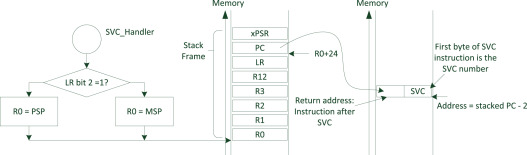
\includegraphics{3-s2.0-B9780124080829000105-f10-05-9780124080829.jpg}
        \caption{SVC\_Handler 初始化流程与异常栈简图}
    \end{figure}

\end{frame}

\begin{frame}
    \frametitle{系统调用}

    本项目实现的系统调用列表:

    \begin{center}
        \begin{tabular}{ |c|c| }
            \hline
            \textbf{系统调用 ID} & \textbf{功能} \\ \hline
            0 & 保留 \\
            1 & 交出控制权并立即执行调度 \\
            3 & Rust 格式字符串打印 \\ 
            4 & C 格式字符串打印 \\
            5 & 进程退出 \\
            6 & 进程创建 \\
            7 & 打印整型数据 \\ \hline
        \end{tabular}
    \end{center}
    
\end{frame}

\begin{frame}

    \frametitle{进程调度}

    本项目通过一个定长数组存放进程控制块,最大可容纳进程数为 11 个,采用时间片轮转调度算法执行调度。

    \par

    进程调度器存放如下状态:

    \begin{center}
        \begin{tabular}{ |c|c|c| }
            \hline
            \textbf{名称} & \textbf{类型} & \textbf{说明} \\ \hline
            is\_activated & bool & 是否完成初始化 \\ 
            current\_process & usize & 当前运行 PID \\ 
            pending\_process & usize & 待决 PID \\ 
            pcbs & PCB[12] & 进程控制块数组 \\ \hline
        \end{tabular}
    \end{center}
    
\end{frame}

\begin{frame}
    \frametitle{进程控制块}

    进程控制块存放以下信息:

    \begin{center}
        \begin{tabular}{ |c|c|c| }
            \hline
            \textbf{名称} & \textbf{类型} & \textbf{说明} \\ \hline
            is\_some & bool & 是否存放有效信息 \\ 
            pid & usize & 进程 ID \\ 
            ppid & usize & 父进程 ID \\
            stack\_base & u32 & 堆栈基地址 \\
            entry\_point & u32 & 进程入口点 \\
            priority & u32 & 进程优先级 \\
            state & ProcessState & 进程状态 \\ 
            running\_state & SavedState & 进程运行态(栈顶地址) \\ \hline
        \end{tabular}
    \end{center}
\end{frame}



\begin{frame}

    \frametitle{进程调度 - 上下文切换}

    按照内核初始化时对 SysTick 的配置,该外设每隔 50ms 将产生一个 SysTick 中断。中断处理器
    检查进程调度器状态,如调度器已完成初始化,则待决一个 PendSV 异常。该异常优先级最低,在完成
    其他所有中断后择机执行。

    \par

    PendSV 异常处理器负责保存当前运行进程状态,从调度器中检出下一个应当运行的进程,恢复该进程的状态并
    将控制权交由目标程序。

    \vspace{0.5em}

    \begin{tikzpicture}[font=\footnotesize]

        \node[box] (EXC) at(0,2) {PendSV 异常};
        \node[box] (SAVEEXTRA) at(3,2) {保存 R4 - R11};
        \node[box] (CHECKINIT) at(6,2) {检查初始化状态};
        \node[box] (CHECKPEND) at(6,1) {检查待决进程};
        \node[box] (INIT) at(9,2) {初始化调度器};
        \node[box] (INITPEND) at(9,1) {初始化待决进程};
        \node[box] (SWITCH) at(9,0) {切换下一进程};
        \draw[->] (EXC)--(SAVEEXTRA);
        \draw[->] (SAVEEXTRA)--(CHECKINIT);
        \draw[->] (CHECKINIT)--(INIT);
        \draw[->] (CHECKINIT)--(CHECKPEND);
        \draw[->] (CHECKPEND)--(INITPEND);
        \draw[->] (CHECKPEND)--(SWITCH);
    \end{tikzpicture}
    
\end{frame}

\begin{frame}

    \frametitle{进程调度 - 中断流程图示}



\end{frame}

\begin{frame}

    \frametitle{进程调度 - 栈内存图示}

\end{frame}

\end{document}
